This question concerns the homogeneous wave equation on an unbounded spatial domain:
          \[ {\d^2 u \over \d t^2} = {\d^2 u \over \d x^2}, 
               \qquad -\infty < x < \infty,  
               \quad   t>0.\]

Find the solution $u(x,t)$ to this equation with 
the following initial conditions:
\begin{enumerate}
\item $u(x,0) = 2 \sin(x)@ e^{-x^2}$, 
      \quad ${\displaystyle{\d u\over\d t}(x,0) = 0}$;

\vspace*{1em}
\item $u(x,0) = 0$, \hspace*{4.5em}
      \quad ${\displaystyle{\d u\over\d t}(x,0) = -{2x\over (1+x^2)^2}}$;

\vspace*{1em}
\item $u(x,0) = 2 \sin(x)@ e^{-x^2}$, 
      \quad ${\displaystyle{\d u\over\d t}(x,0) = -{2x\over (1+x^2)^2}}$. 

\vspace*{1em}
\item Produce a plot (or plots) showing your solution to part~(c) over $-10\le x \le 10$\\
      at times $t=0, 1, 2, 3, 4, 5$. 
\end{enumerate}

%%%%%%%%%%%%%%%%%%%%%%%%%%%%%%%%%%%%%%%%%%%%%%%%%%%%%%%%%%%%%%%%%%%%%%%%%%%%%%%%

\ifthenelse{\boolean{showsols}}{\begin{solution}
\begin{enumerate}
\item D'Alembert's solution takes the form
      \begin{eqnarray*}
            u(x,t) &=& {\textstyle{1\over2}}\big(\psi(x-t) + \psi(x+t)\big) \\[0.5em]
                   &=& \sin(x-t) e^{-(x-t)^2} + \sin(x+t) e^{-(x+t)^2}.
      \end{eqnarray*} 
\item D'Alembert's solution is now
        \[  u(x,t) = {\textstyle{1\over2}}\int_{x-t}^{x+t} \gamma(s)\, ds.\]
      We can compute
        \[ \int -{2x \over (1+x^2)^2} \, dx = {1\over 1+x^2} + {\rm constant},\]
      and so 
      \begin{eqnarray*}
            u(x,t) &=& {\textstyle{1\over2}}
                        \big(\psi(x-t) + \psi(x+t)\big) \\[0.5em]
                   &=& {\textstyle{1\over2}}
                        \Big( {1\over 1+(x+t)^2} - {1\over 1+(x-t)^2}\Big).
      \end{eqnarray*} 

\item When the nonzero boundary conditions from (a) and (b) are combined, 
      we simply sum the solutions to the two previous parts:
\[ u(x,t) = \sin(x-t) e^{-(x-t)^2} + \sin(x+t) e^{-(x+t)^2}
               + {\textstyle{1\over2}}
                  \Big( {1\over 1+(x+t)^2} - {1\over 1+(x-t)^2}\Big). \]


\item The following plots show the solution in part~(c) at times $t=0,1,2,3,4,5$,
      with the code that produced the plots following.

\newpage
      \begin{center}
          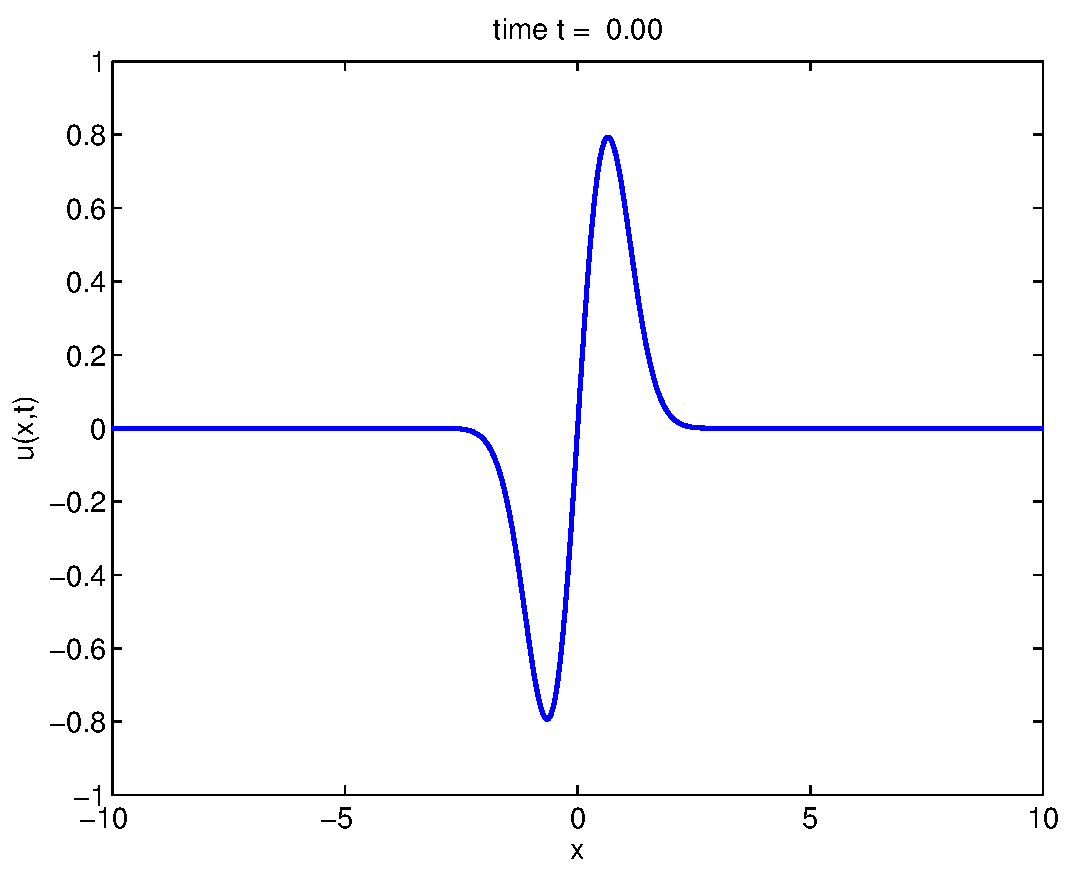
\includegraphics[scale=0.36]{dalembert0}\quad
          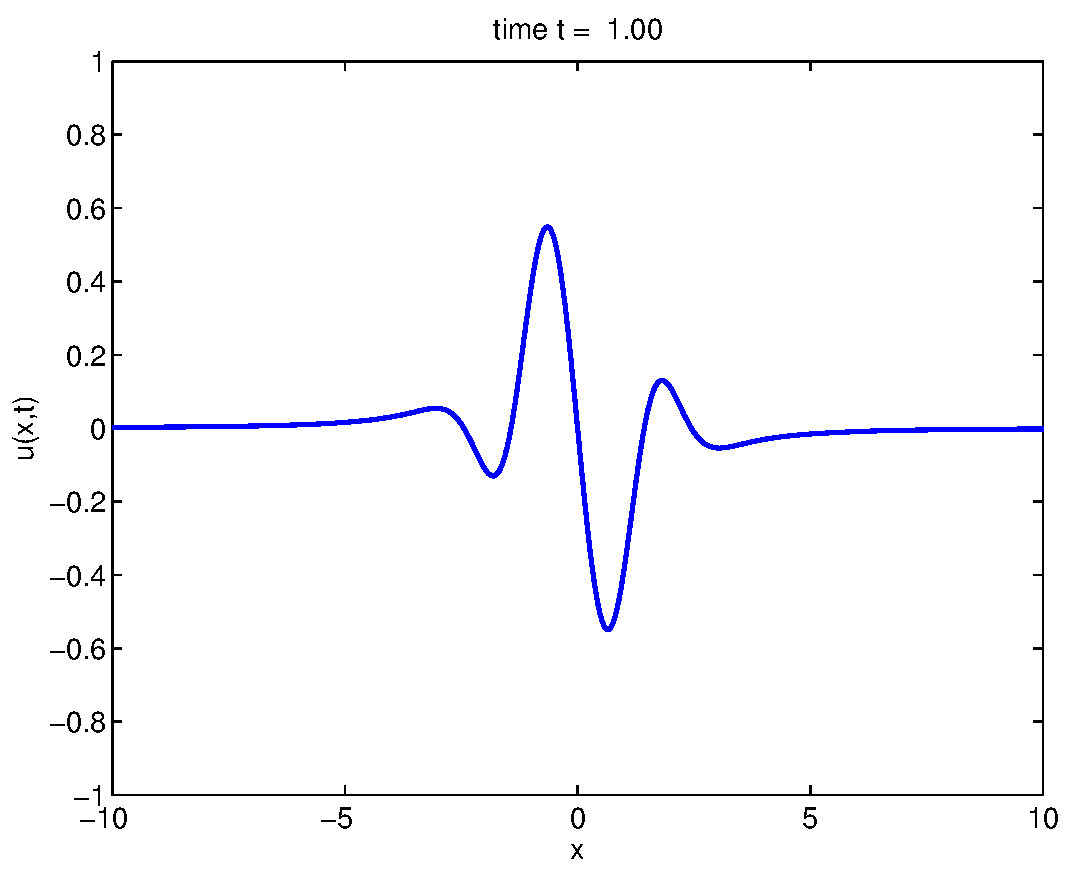
\includegraphics[scale=0.36]{dalembert1}

          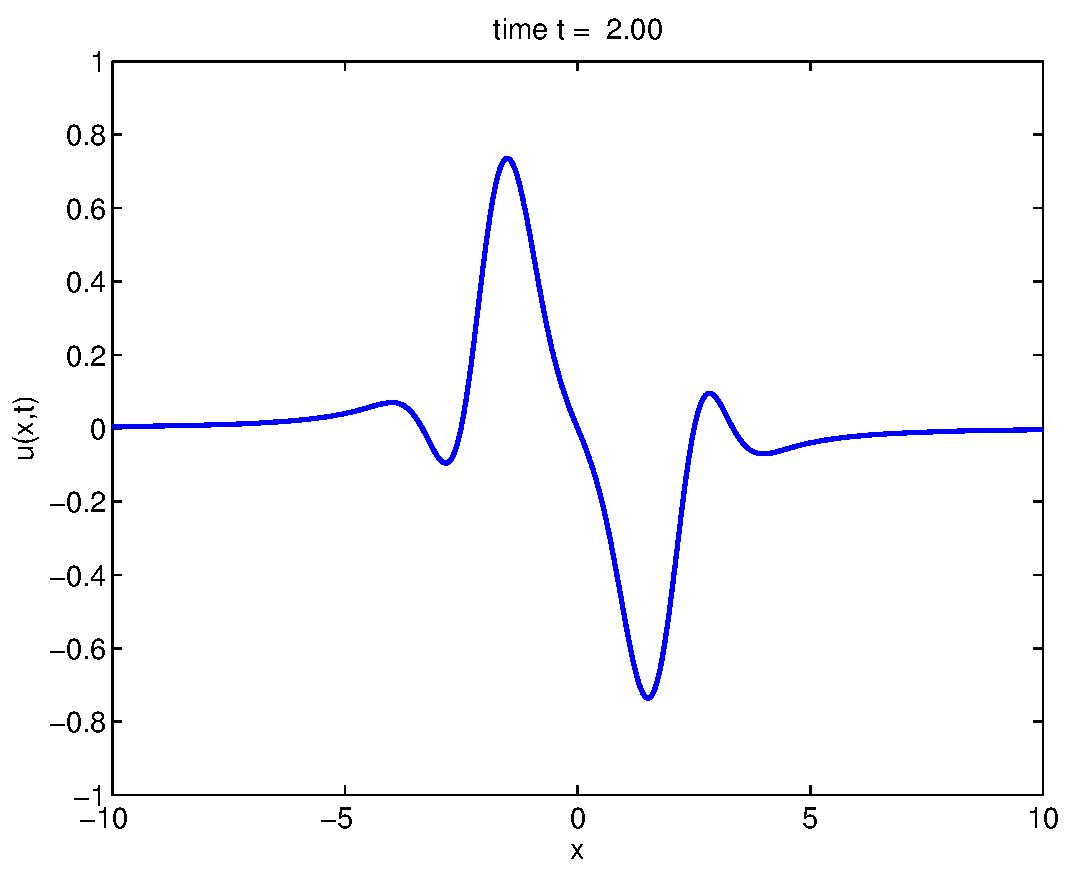
\includegraphics[scale=0.36]{dalembert2}\quad
          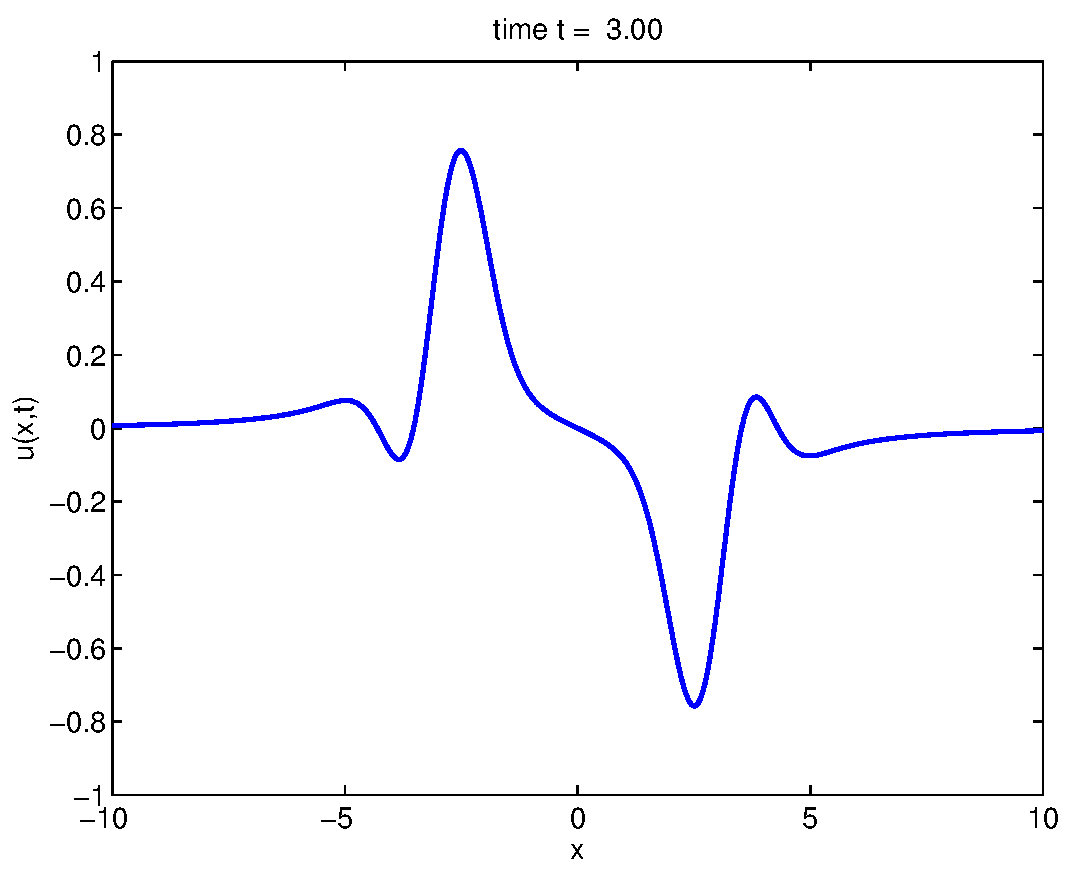
\includegraphics[scale=0.36]{dalembert3}

          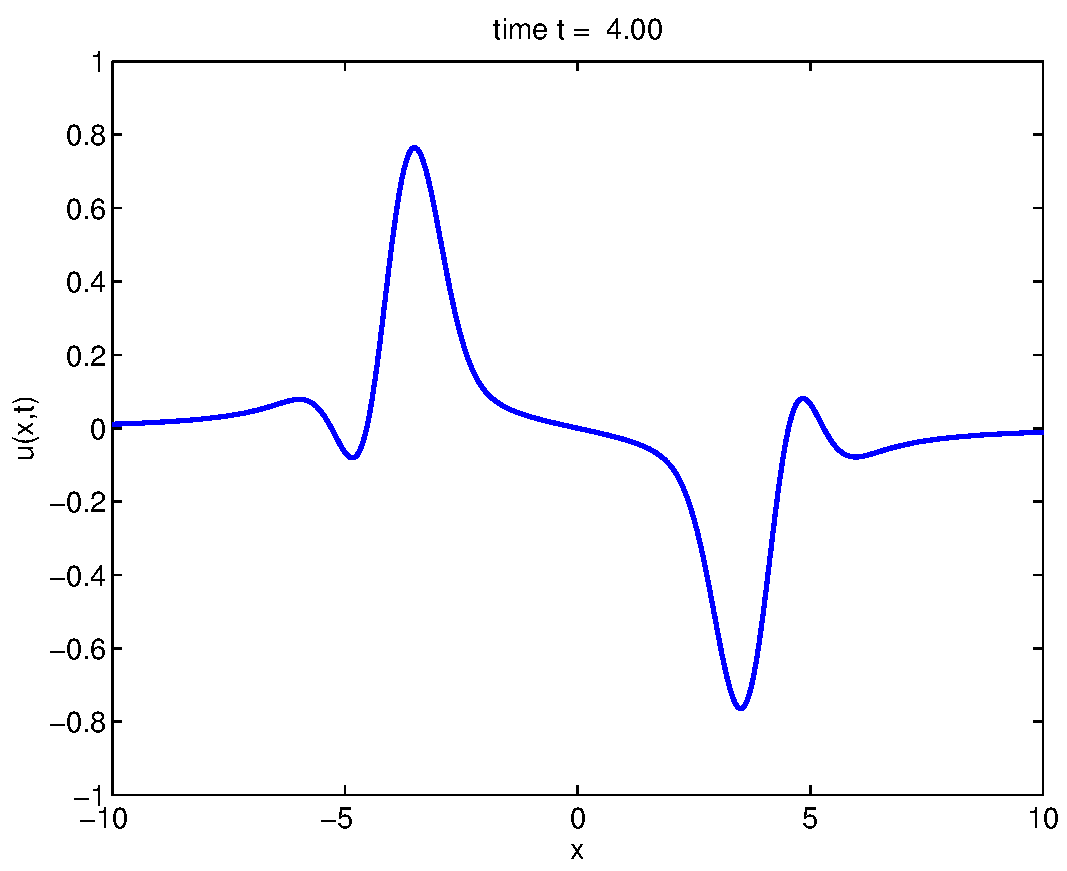
\includegraphics[scale=0.36]{dalembert4}\quad
          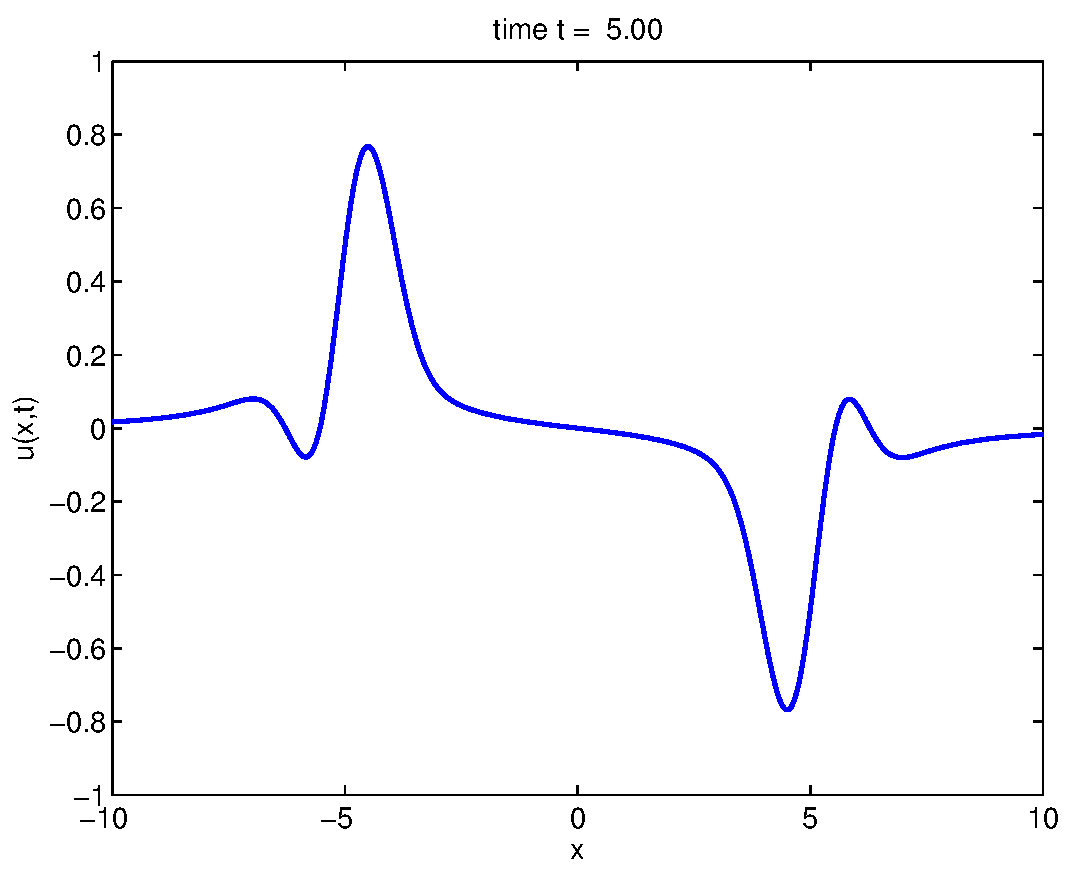
\includegraphics[scale=0.36]{dalembert5}
      \end{center}

      \input dalembertcode
\end{enumerate}
\end{solution}}{}

